\chapter{Project Plan}

This section contains ideas on distributing work across the project, including the estimates for milestone completions.
Of course, estimating the complexity of an unknown problem is very challenging, so this section will also highlight which tasks may be omitted and include relevant extensions in case the actual project timeline allows for more/less work completed.\\

A portion of the work was completed before the interim report deadline. It is the following:

 - Concept generalisation dataset generation and cleaning. A few hundred concept generalisation examples were constructed using the available atomic sentences from the dataset. This dataset is also cleaned to remove incorrect atomic sentences.
 
 % TODO reference
 - Got familiar with the tools and techniques that will be used. In particular, I have greatly improved my knowledge of Answer Set Programming \cite{RefWorks:RefID:1-lifschitz2008answer}, spacy \cite{RefWorks:RefID:24-spacy} library and ILASP \cite{RefWorks:RefID:18-law2020ilasp} platform. The familiarisation also involved looking into other inductive logic programming frameworks like FastLAS \cite{RefWorks:RefID:19-law2020fastlas:}. 

 - Hand-crafted syntactic concept generalisation solution creation. The logic-based learning systems such as ILASP need an inductive bias used as a search space. So, creating a simple hand-crafted solution can help design the inductive bias for the system and serve as a benchmark of the performance of such a system. This work also involved the design of the knowledge representation.\\
 
 
The upcoming work has two major development milestones: completion of the syntactic concept generation and the atomic sentence generation.
Additionally, the 3rd large milestone would involve the generation of the explanations for the task.
The project may not reach this milestone depending on the success of the first two.
To accommodate the possibility that the milestones might be completed earlier than possible, two extensions are proposed: hierarchical concept extraction, concept linking across sentences and semantical concept extraction.
The hierarchical concept would involve creating a notion of a hierarchy between extracted concepts and utilising that information to make predictions.
On the other hand, concept linking across sentences would include a way to associate terms which occur in different sentences. For instance, in a pair of sentences \emph{Obama is a former US president. He finished his term in 2017.}, he could be linked to Obama.
Finally, the semantical concept extraction would involve extracting only relevant sentences for a given problem, such as a sentence \emph{The batter hit the ball} within the context of baseball.

\begin{landscape}

The current plan below involves general task descriptions, when they will be worked on and red lines indicating when the milestones will be completed. 
The following figure proposes a project plan and the tasks that will be attempted each week.

The project plan is shown in \ref{project-plan}. It gives rough estimates of dates when I plan to work on each specific project part.
This plan was designed with the following constraints in mind:

 - The research needs to be done early so that informed design decisions can be made.
 
 - It is expected that the atomic sentence generation is the most complex part of the project, followed by the concept generalisation implementation.
 
 - In the spring term, two week period allows for more work than the same period in the autumn term. 
 It is a consequence of taking three modules instead of four.
 Moreover, the summer term is completely available for project work, so two week period should be more productive than the same period in the spring term. Hence, the generation of atomic sentences has fewer regions shaded in than the concept generalisation despite being more complex.
 

\begin{figure}[h]
\caption{Project plan. Shaded areas represent times when I plan to be working on a specific part of the project.}
\centering
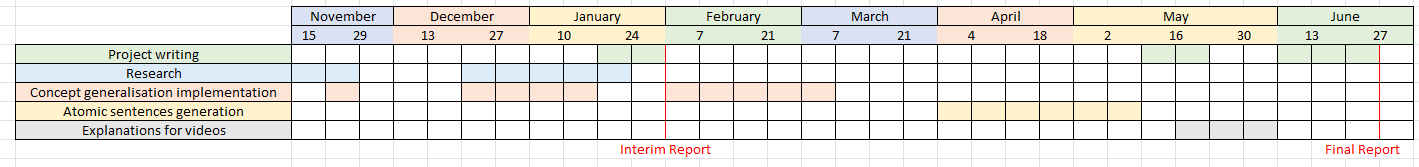
\includegraphics[width=1.6\textwidth]{project/project plan.PNG}
\label{project-plan}
\end{figure}


\end{landscape}